
\def\covmac{/Users/matiascovarrubias/Documents/universidad/NYU/Research/Repositories/marketsAI/marketsai/Documents/Figures}
\let\dir=\covmac

\documentclass[11pt,english]{article}
\usepackage[T1]{fontenc}
\usepackage[latin9]{inputenc}
\usepackage{geometry}
\geometry{verbose,tmargin=1in,bmargin=1in,lmargin=1in,rmargin=1in}
\usepackage{enumitem}
\usepackage{amsmath}
\usepackage{amssymb}
\usepackage{setspace}
\usepackage[authoryear]{natbib}
\onehalfspacing

\makeatletter
%%%%%%%%%%%%%%%%%%%%%%%%%%%%%% Textclass specific LaTeX commands.
\newlength{\lyxlabelwidth}      % auxiliary length 

%%%%%%%%%%%%%%%%%%%%%%%%%%%%%% User specified LaTeX commands.
% Added by lyx2lyx
%  for proper underlining
\PassOptionsToPackage{normalem}{ulem}
\usepackage{ulem}
\let\cite@rig\cite
\newcommand{\b@xcite}[2][\%]{\def\def@pt{\%}\def\pas@pt{#1}
  \mbox{\ifx\def@pt\pas@pt\cite@rig{#2}\else\cite@rig[#1]{#2}\fi}}
\renewcommand{\underbar}[1]{{\let\cite\b@xcite\uline{#1}}}

\usepackage{tikz}
\usetikzlibrary{arrows,snakes,shapes,calc}
\usepackage{pgfplots}
\usepackage{color}
\definecolor{darkred}{rgb}{0.8,0.1,.3}

%\usepackage[pagebackref=true]{hyperref}
\usepackage{hyperref}
\hypersetup{
    colorlinks,
    citecolor=blue,%
    filecolor=black,%
    anchorcolor=darkred,
    linkcolor=darkred,%
    urlcolor=cyan
}

\usepackage[titletoc,toc,title]{appendix}
\usepackage{colortbl}
\usepackage[bottom]{footmisc}
\usepackage{hhline}

% For auto-creation of tables
\usepackage{amsmath,amsthm, graphicx, setspace, booktabs, tabularx, subcaption}
\usepackage{amsfonts, fancyhdr, epstopdf, color, verbatim, pdflscape}
\usepackage[font=small,format=plain,labelfont=bf,textfont=it]{caption}
\usepackage{times}
\makeatother
\usepackage{babel}

% new commands
\newcommand{\E}{\mathbb{E}}

\begin{document}
\title{Deep Reinforcement Learning in Macroeconomic Models}
\author{Matias Covarrubias}
\maketitle
\begin{abstract}
Can artificial intelligent (AI) algorithms learn optimal intertemporal behavior without knowing any mathematical details of the economy beforehand?  How should we specify economies and markets so as to make them easy to learn? In this paper, I apply Deep Reinforcement Learning (Deep RL), the current front-runner in the design of AI agents, to macroeconomic problems. In the context of an investment under uncertainty model with heterogenous agents, I show that Deep RL agents can learn the rational expectations solution and I suggest design choices that aid such learning. Then, by manipulating our baseline framework I highlight three topics in which this technology can be useful: high dimensional problems, incomplete information problems and equilibrium selection in models with multiple equilibrium.
\end{abstract}

\newpage 
\section{Introduction}

\begin{itemize}
		\item {\color{red} To do: 
		
		\begin{itemize}
			\item Present the RL framework as having three distict characteristics: model-free, sample or simulation based, and using deep neural nets.
			\item Explain why neural nets help based on the notes you saw. Be fast about it.
			\item Reintoriduce as a "learning in macro" paper.
	\end{itemize}}

	\item Paragraph 1 (reframe) :Can artificial intelligent (AI) algorithms learn optimal intertemporal behavior without knowing any mathematical details of the economy beforehand?  How should we specify economies and markets so as to make them easy to learn? In this paper, I apply Deep Reinforcement Learning (Deep RL), the current front-runner in the design of AI agents, to macroeconomic problems. In the context of an investment under uncertainty model, I show that Deep RL agents can learn the rational expectations solution and I suggest design choices that aid such learning. Then, by manipulating our baseline framework I highlight three topics in which this technology can be useful: high dimensional problems, incomplete information problems and equilibrium selection in models with multiple equilibrium.\medskip
	
	\item Paragraph 2: Explain model free RL. \medskip 
	
	\begin{itemize}
		\item RL is a class of algorithms that adapt dynamic programming techniques such as value function and policy function iteration to the problem of online learning, that is, to learn how to control a system by interacting and experimenting with it. Other historical names for this method are approximate dynamic programming, learning based control and automated optimization.  \medskip
		\item A key characteristic of RL algorithms is that they do not use any mathematical knowledge of  the system they are controlling, other than the allowed actions and states. They feed actions to the system and observe the reward they get that period and how the state evolves. After millions of such transitions, if learning is successful, they are able to estimate the consequences of their actions accurately and thus make optimal decisions. \medskip
	\end{itemize}

	\item Paragraph 3: Deep RL and the advent of this technology. \medskip 
	
			\begin{itemize}
			\item Deep RL adds neural nets as function approximator. Explain \citet{mnih2013} paper. \medskip
			\item Why it has been so effective? Scalability and computation power. \medskip
			\item Success cases: games, robotics, self-driving vehicles, industrial optimization. 
		\end{itemize}

	\item Paragraph 3: Traditional challenges of Deep RL and why economics may be particularly well suited for this technology.\medskip
	
	\begin{itemize}
		\item Rewards engineering is usually the main bottleneck. In many problems, such as games or robotics, you only get positive rewards after successfully achieving some final objective, so the researcher needs to design signals to indicate to the agents whether they are making progress or not. In economics, rewards are well specified in every period. \medskip
		
		\item Also, RL algorithms usually require millions of transitions in order to learn, which may be computationally expensive. This problem is very serious in environments with high dimensional states, such as images, and with complex transitions logic, as in the case of games or robotics. In economics, sampling a transition is usually very fast, as we are only dealing with vectors whose transitions laws can be expressed with simple mathematical functions. \medskip
		
		\item Finally, in many problems the algorithms get stuck in local optima. While this is also a potential problem in complex economic models, for many models we have nice regularity properties. \medskip
	\end{itemize}
	

	\item Paragraph 5: But, economic problems present their own challenges. \medskip
	
	\begin{itemize}
		\item Markets are a multi-agent problem. While multi agent Deep RL is a very active topic with some impressive success cases, it faces a crucial challenge: agents learn and explore while other agents learn and explore. This means that the environment is non-stationary and at the beginning it may be very chaotic. Whether order arises from such chaos is an empirical question with no theoretical guarantees. \medskip
		
		\item In economics, rigorous insights often rely on exact solutions. That is, we are trying to solve very precise control problems, so usual assumptions such as discrete action spaces may not be satisfactory. Deep RL agents might get a very high percentage of the optimal discounted utility, but the solution may still lack some of the qualitative features of the exact solution. Example: growth model with fixed saving rate instead of decreasing saving rate. \medskip
	\end{itemize}

		\item Paragraph 4: Explain why this could be useful besides the study of learning in macroeconomics: \medskip 
	
	\begin{itemize}
		\item With this technology, we only need to specify the economy's action space, observation space, initial state and transition laws. This makes it simple to setup an economy on which Deep RL agents can learn. \medskip
		
		\item The algorithm's structure is mostly the same regarding the problem at hand. The algorithm only needs to adapt the dimensions of its function approximators (e.g., neural nets) to the state space and action space of the environment, which can be easily automated. Thus, the same algorithm can learn to play chess or to calculate optimal saving behavior. As a corollary, the information available to each agent can be manipulated easily, without making any changes to the algorithm. Also, different versions of the economy can be constructed without need to recalculate the set of equations that describe the optimal solution  \medskip
	\end{itemize}

	\end{itemize}

	\subsection{Preview of leading framework and exercises} 
	
	\begin{itemize}
	
	\item {\color{red} To do: 
	
\begin{itemize}
	\item Re-sell the model as a version of the stochastic growth model with heterogeneous agents. 
	\item Fill exercisez. Re-wrtie the role that each plays. For exercise 2, two roles: multi-agent and strategic behavior.
	\item Write results very minimallisticaly. 
\end{itemize}}
	\item My criteria for choosing a baseline framework are the following:
	
	\begin{itemize}
		\item Simple economics, challenging solution: the problem should be easy to explain and with clear economics. Nevertheless, the control problem should be challenging. \medskip
		
		\item Dynamics at the forefront: the key trade-offs of the model should be intertemporal, since we are interested in the application of deep RL to dynamic problems. \medskip
		
		\item Meaningful scalability: the problem needs to have a clear path to scalability in which the dimensionality truly affects the economics of the problem. As such, it cannot have aggregation properties, so each variable in the state space should affect optimal behavior. \medskip
	\end{itemize}

	\item Consistent with this criteria, I present a model of investment under uncertainty in which we focus on the purchase market for capital goods. There are a discrete number of buyers (household who produce, consume and invest) and sellers (each producing a different type of capital good). More precisely:
	

	\item $N^h$ households indexed by  choose how much to consume and how much to invest in order to maximize the discounted intertemporal utility.\medskip
	
	\item The final good is produced using $N^c$ capital goods. All capital goods are bundled with a Cobb-Douglas aggregation and the production function have decreasing returns to scale over that bundle. The  total factor productivity of each households follows a markov chain.   \medskip
	
	\item The agent allocates current production between consumption and investment in new capital goods. The cost in term of the final good of producing  new capital goods  is quadratic in investment.  \medskip
	
	\item  We will consider both a  market's formulation and a planner's formulation of the problem. In the market formulation, for each capital good there is a firm who pays the quadratic cost and sells the capital good. In the planner formulation, the planner decides how much of the final good to allocate in each capital good for each household, and investment is determined by how many units can be produced given the total allocation of resources by all households on that capital good. 
	
	\item Within this framework we perform the following exercises:
	
	\begin{itemize} 
		\item Exercise 1: The planner problem. For single agent problems, we can ask the Deep RL agents to solve the exact same problem we formulate in macroeconomic models. Thus, we can check how close does the Deep RL agent gets to the solution obtained by classical dynamic programming methods. If convergence is achieved, we confirm that the expectations implicit in the behavior of the Deep RL agent  are rational. Also, we can scale the problem to many state variables and evaluate the potential of this learning methodology to deal with high dimensional dynamic control problems. \medskip
		
		\item Exercise 2: Many households. In order to evaluate the ability of deep RL agents to learn in multi-agent environments, we consider the problem of many households who need to purchase capital goods from the capital good firm. The supply side stays competitive, that is, the price paid by households correspond to the marginal cost evaluated at the aggregate demand level. In this formulation, the deep RL solution differs from the competitive market solution because agents do not assume that the price they pay is independent of the actions. In the tradition competitive equilibrium formulation, we impose such price-taking behavior by taking the price as given when we calculate the first order conditions. In the RL formulation, we do not use first order conditions. Instead, we formulate the economy as a markov game, in which the consequences of actions are well specified for any behavior, optimal or not. Within this formulation, we increase the number of households to evaluate whether a larger number of buyers increase competition on the demand side and thus increase quantity purchased. In the limit, the solution should approximate the competitive solution.   \medskip
		
		\item Exercise 3: Incomplete Information. In order to showcase the flexibility with which we can manipulate the information structure of the economies under study, we simulate an economy with many households in which half of the households observes the stock and idiosyncratic shock of all households, and the other half only observes his own state and aggregate statistics of other households state variables. With this exercise, we can calculate the increase in expected utility from having the extra information, and compare the investment behavior. \medskip
		
		\item Exercise 4: AI agents in both supply and demand. Finally, I  simulate an economy in which both sellers and buyers are Deep RL agents. This is challenging because we cannot make use of a "walrasian auctioneer" that take magnets first order conditions and determine prices by solving a system of equations. Also ,we can study the strategic behavior of agents by varying both the number og sellers and buyers. \medskip
		
		
		
		
	
	\end{itemize}

	
	\item Results
	
\end{itemize}
	
	\subsection{Related Literature}


	\begin{itemize}
			
		\item {\color{red} To do: 
			
			\begin{itemize}
				\item Fill with bullet-points. 
				\item Put paper on macro and machine learning in perspective. (just bullet points)
		\end{itemize}}
	
		\item paragraph 1: Learning in Macroeconomics. \medskip
		
		\item paragraph 2: Reinforcement Learning in economics. \medskip
		
		\begin{itemize}
			\item \citet{calvano2020} study algorithmic collusion by evaluating the behavior of q-learning algorithms, the most classical RL algorithm, when they compete in a repeated static game consisting on a differentiated bertrand with constant marginal costs. They show that algorithms learn to collude, in the sense that they charge a markup that is above the static nash solution, even though it is not as high as the monopolistic solution. Their problem, though repeated, is static in the sense that there is no state variable nor inter-temporal choice. 
			
			\item \citet{asker2021} study a similar problem as \citet{calvano2020} but their focus is on how the specific RL algorithm affect the collusive behavior. They also use first generation reinforcement learning algorithms.
			
			\item \citet{graf2021} also study algorithmic collusion but with a deep reinforcement learning algorithm that can be used on environments with continuous action and observation space.
			
			\item 
			
		\end{itemize}
		
		\item paragraph 3: Literaure on machine learning learning for high-dimensional problems.
	\end{itemize}
	

\section{A Primer on Reinforcement Learning}




\begin{itemize}
	\item {\color{red} To do: 
	
	\begin{itemize}
		\item 1 paragraph defining markov problems very minimallistically. 
		\item Just small phrases with the flow of the arguments.
		\item Explain soft -actor critic algorithms.
\end{itemize}}
\item Define Markov Decision Problems.
\item Example 1: Monopolist problem.
\item Algorithm: Q-learning
\begin{itemize}
	\item We start from simplest single agent algorithm. The problem is: \medskip
	$$\underset{a \in A}{\max} \sum_{t=s}^{\infty} \gamma^{s-t} E_t[r_{t+s}]$$
	
	\item Two value functions: \medskip
	\begin{enumerate}
		\item state-value function: $V(s)=\max_{a\in A} \{E[r|s,a] + \gamma E[V(s')|s,a] \}$ \medskip
		\item action-value function: $Q(s,a)=E(r|s,a)+\gamma E[\max_{a'\in A} Q(s',a')|s,a]$ \medskip
	\end{enumerate}
	\item Q-Learning:  \medskip
	\begin{itemize}
		\item Initialize $Q_0(s,a)$. Loop until converge:  \medskip
		\begin{itemize}
			\item agent chooses $a= \text{arg} \max Q(s,a)$  and observes $\{r, s'  ,s, a\}$. \medskip
			\item Old Q: $Q(s,a)$. \medskip
			\item  Target Q: $r_t+\gamma \max_{a' \in A} Q(s',a')$. \medskip
			\item New Q: $$Q'(s,a)=(1-\alpha) Q(s,a) +\alpha [r+\gamma \max_{a' \in A} Q(s',a')]$$ \medskip
		\end{itemize}
	\end{itemize}
\end{itemize}

		\item Both in theory and in practice, one of the most important ingredients for successful learning is exploration. Agents do not always act according to what they currently believe to be optimal but they sometimes choose actions at random in order to learn. How much exploration to perform is an open problem, called the exploration-exploitation dilemma. \medskip
\item Proof of convergence and theory.
\begin{itemize}
\item \citet{tsitsiklis1994} perform an extensive convergence analysis of q-learning algorithms. His proof of convergence is based on contraction mapping theorem.
\item \citet{bertsekas2012} introduce a mix of policy iteration and q-learning
that improves efficiency even for approximate methods. It seems great
check it.
\item \citet{ma2020} show formally that the recursive specification of
the q values can be considered as a transformation of the bellman
operator. The authors use this q-transform to solve problems with
unbounded rewards.
\item \citet{ma2021} use computational complexity theory and numerical
experiments to conclude that the q-transform leads to gains in computational
efficiency. NOTES: WHY?


\end{itemize}
\end{itemize}

\subsection{Deep Reinforcement Learning}

\begin{itemize}
	\item Deep Q Network (DQN)
	\begin{itemize}
		\item DQN consists in approximating the Q function with a neural net: $\hat{Q}(s,a) \equiv  \mathcal{N}_\rho \sim Q(s,a)$.\medskip
		\item The parameters $\rho$ are estimated in order to minimize\medskip
		$$\mathcal{L}(\rho)=\E \left[ \left(\hat{Q}(s,a)-(r_t+\gamma \max_{a' \in A} \hat{Q}(s',a')) \right)^2 \right] $$
		
		in observed transitions $\{r, s'  ,s, a\}$ .\medskip
		
		\item The most widely used NN is a composite function made of nested linear functions:  \medskip
		
		$$\mathcal{N}_\rho (x)=\sigma_K(W_K ... \sigma_2(W_2 \sigma_1(W_1x+b_1)+b_2)...+b_K)$$
		
		where $x$ is the input (in our case the transitions $\{r, s'  ,s, a\}$), $W_i \in \mathbb{R}^{m_{i+1}\times m_i}$ are the weights, $b_i \in \mathbb{R}^{m_i+1}$ are the biases, and $\sigma()$ are activation functions.
	\end{itemize}

	\item Theory: explain proofs by \citet{maei2009}.

\subsection{State of the Art Algorithms}

	\item Before, we gobtaingin a policy by choosing the action that maximizes a parametrized action-value functions. For policy gradient methods, we parametrized the policy directly:
	
	\begin{align*}
	\pi(a,s) = P(a| s, \theta)
	\end{align*}
	
	\item Three reason to consider Policy based methods:
	
	\begin{itemize}
		\item There may situation in which storing the value function may be hard but the policy may be simple.
		\item Another reson why it may be better to use policy gradient is that they have better convergence properties. Value function methods sometimes go wild. 
		\item So there are cases in which the policy may be more compact. Another big one is that these methods work better at continuous or large state spaces, since they circumvent the need to calculate the max over Q. That may be very intensive. This last one may be the bigger one.
		\item We can estimate stochastic policies. 
	\end{itemize}  

	\item Disadvantages:
	\begin{itemize}
	\item  BUT, they are less sample efficient. Maximizing the Q-value is very aggressive, you are trying to summarilze all your current info. 
	\item They typically converge to local rather than global maximum.
	\end{itemize}
	\item Proximal Policy Optimization \citet{schulman2017} is a policy gradient algorithms that has been used in many of the recent success cases (cite all). The first step is to comput an estimator of the policy gradient:
	
	\begin{align*}
	\hat{g} = \hat{\E}_t\left[ \Delta_\theta \log \pi_\theta(a_t | s_t) \hat{A}_t \right]
	\end{align*}
	
	where $\hat{\E}_t$ is the empirical average over a finite batch of transitions. 
		
	\item We transform this estimate in a loss function so we can apply grandient ascent. The loss function is :
	
	\begin{align*}
	L^{PG}(\theta) =  \hat{\E}_t\left[ \log \pi_\theta(a_t | s_t) \hat{A}_t \right]
	\end{align*}
\end{itemize}



\subsection{Multi-Agent Reinforcement Learning}

\begin{itemize}
\item Define Partially Observed Markov Games.
\item Example 1: Algorithmic Collusion.
\item Algorithm: Independent learning.
\item Challenges of multi-agent.
\item Soutions: QMix and other algorithms. 
\item Prominent success cases:
\begin{itemize}
	
\item \citet{berner2019} achieve super-human performance at the game Dota 2. The game is challenging for multiple reasons. It is multi-agent, stochastic, it has a large action and observation space and it requires long term strategy. They authors used a single neural net to approximate both the value function and the policiy function. In particular, they used a single-layer 4096-unit LSTM.

\item \citet{baker2019} show that agents self-playing hide and seek in a complex environment exhibit emergent curricular learning, in which they progressively discover strategies and then device counter-strategies. They use PPO with GAE. The distributed computation framework is called rapid. 
\item \citet{vinyals2019} achieve grand-master level at the game StarCraft 2. ``Observations of player and opponent units are processed using a self-attention mechanism. To integrate spatial and non-spatial information, we introduce scatter connections. To deal with partial observability, the temporal sequence of observations is processed by a deep long short-term memory (LSTM) system. To manage the structured, combinatorial action space, the agent uses an auto-regressive policy and recurrent
pointer network.''. ``For every training agent in the league, we run 16,000 concurrent StarCraft II matches and 16 actor tasks (each
using a TPU v3 device with eight TPU cores23) to perform inference. The game instances progress asynchronously on preemptible CPUs (roughly equivalent to 150 processors with 28 physical cores each), but requests for agent steps are batched together dynamically to make efficient use of the TPU. Using TPUs for batched inference provides large efficiency gains over previous work14,29. Actors send sequences of observations, actions, and rewards over the network to a central 128-core TPU learner
worker, which updates the parameters of the training agent. The received data are buffered in memory and replayed twice. The learner worker performs large-batch synchronous updates. Each TPU core processes a mini-batch of four sequences, for a total batch size of 512. The learner processes about 50,000 agent steps per second. The actors update their copy of the parameters from the learner every 10 s. We instantiate 12 separate copies of this actor--learner setup: one main agent, one main exploiter and two league exploiter agents for each StarCraft race. One central coordinator maintains an estimate of the payoff matrix, samples new matches on request, and resets main and league exploiters. Additional evaluator workers (running on the CPU) are used to supplement the payoff estimates. See Extended Data Fig. 6 for an overview of the training setup.''
\end{itemize}
\end{itemize}


\section{Baseline Framework}

 {\color{red} To do: 
	
	\begin{itemize}
		\item Divide between main text and appendix. Focus only on what's important. 
\end{itemize}}


\begin{itemize}
	\item $N^h$ households indexed by $i$ choose how much to consume and how much to invest in order to maximize $\sum_{t=0}^{\infty} \beta^t U(C_{i,t})$.\medskip
	
	\item The final good is produced using $N^c$ capital goods indexed by $j$ according to technology $$Y_{i,t}=Z^h_{i,t} \left(\Pi_{j=1}^{N^c} K_{i,j,t}^{1/N^c} \right)^{\alpha} = Z^h_{i,t} \Pi_{j=1}^{N^c} K_{i,j,t}^{\alpha/N^c}$$  where total factor productivity $Z^h_{i,t}$ follows the stochastic process $Z^h_{i,t+1} \sim \mathcal P(Z^h_{i,t})$. We assume that $\alpha<1$ in order to avoid having aggregation, that is, given decreasing returns to scale the distribution of capital stocks matters.  \medskip
	
	\item The agent allocates $Y_{i,t}$ between consumption and investment in new capital goods. The evolution of the stock of capital is 
	
	$$K_{i,j,t+1} = (1-\delta) K_{i,j,t} + I^h_{i,j,t}$$ 
	
	where $I^h_{i,j,t}$ represents investment in capital good $j$ by household $i$ in period $t$\footnote{The superscript $h$ is added because we will consider both planner and market solutions to the problem, and in the latter it is useful to keep track of the agent that is choosing the variable $I$.}. 
	
	\item The cost in term of the final good of  producing $I^h_{j,t}$ new units of capital good $j$  is $\frac{\phi}{2} \left(I^h_{j,t}\right)^2$.  \medskip
	
	\item In order to frame the problem, we define the saving rate $s_{j,t}$ as the expenditure on new capital goods $j$ in terms of the final good. Thus, consumption is 
	
	$$C_{i,t}=(1-\sum_{j=1}^{N^c} s_{i,j,t})Y_{i,t}$$ 
	
	\item We will consider both a competitive market's formulation and a planner's formulation of the problem: 
	
	\begin{itemize}
		\item First, we assume that there is a market for investment goods and we introduce capital good firms that pay the adjustment cost and sell the investment good at price $p^k_{j,t}$. Thus, from the point of view of the household, investment is $I^h_{i,j,t} = s_{i,j,t}/p^k_{j,t}$.   \medskip
		
		\item Second, in order to formulate the planner's problem, we assume that all the resources that are committed by households for investment on capital good $j$ are actually employed in production, and then total production of capital good $j$ is distributed among housholds according to their contribution. In this case, total production is defined implicitly by:
		
		$$\sum_{i=1}^{N^h} s_{i,j,t} Y_{i,t} = \frac{\phi}{2} I_{j,t}^2 \quad \text{for } j \in [1,...,N^h]$$
		
		Solving for $I_{j,t}$ we get:
		
		$$I_{j,t} =  \sqrt{\frac{2}{\phi} \sum_{i=1}^{N^h} s_{i,j,t} Y_{i,t}}$$
		
		We can then distribute it among households according to
		
		$$I_{i,j,t} = \frac{s_{i,j,t}Y_{i,t}}{ \sum_{i=1}^{N^h} s_{i,j,t} Y_{i,t}}  I_{j,t} =   \frac{s_{i,j,t}Y_{i,t}}{\sqrt{\frac{\phi}{2} \sum_{i=1}^{N^h} s_{i,j,t} Y_{i,t}}}$$
		
	\end{itemize}  
\end{itemize}


\subsection{Competitive Market's Formulation}

\begin{itemize}
	\item Now we have two types of agents.  The household purchases capital goods and consume the final good.  The capital good firm, which produces the capital good subject to a quadratic cost. 
\end{itemize}

\subsubsection{Household}
\begin{itemize}
	
	\item The recursive formulation of the problem for household $i$ is:
	
	
	\begin{align*}
	V_i \left(\{K_{i,j,t}\}_{i,j}\right) = &\max_{\{s_{i,j,t},K_{i,j,t+1}\}_{j}}  U(C_{i,t}) + \beta \E_t V_i(\{K_{i,j,t+1}\}_{i,j}) \qquad \text{s.t.}\\
	&\qquad
	C_{i,t} = (1-\sum_{j=1}^{N^c} s_{i,j,t})Y_{i,t} \\
	&\qquad
	Y_{i,t}=Z^h_{i,t} \Pi_{j=1}^{N^c} K_{i,j,t}^{\alpha/N^c}\\
	&\qquad
	K_{i,j,t+1} \leq (1-\delta) K_{i,j,t} + \frac{s_{i,j,t} Y_{i,t}}{p^k_{j,t}}  \quad \text{for } j \in [1,...,N^c] 
	\end{align*}
	
	
	\item The lagrangian of the problem is: 
	
	\begin{align*}
	\mathcal{L}_{t} &= \E_t \sum_{r=0}^{\infty}\beta^r  \left( U\left( (1-\sum_{j=1}^{N^c} s_{i,j,t+r})Z^h_{i,t+r}\Pi_{j=1}^{N^c} K_{i,j,t+r}^{\alpha/N^c}  \right) + \right. \\
	& 	\left. \sum_{j=1}^{N^c}  Q_{i,j,t+r} \left[(1-\delta) K_{i,j,t+r} +\frac{s_{i,j,t+r}Z^h_{i,t+r} \Pi_{j=1}^{N^c} K_{i,j,t+r}^{\alpha/N^c}}{p^k_{j,t+r}} -K_{i,j,t+r+1}\right] \right)
	\end{align*}
	
	\item The first order conditions are:
	
	\begin{align*}
	& \left[s_{i,j,t}\right] && Q_{i,j,t}  =p^k_{j,t} U'(C_{i,t}) \\
	& \left[K_{i,j,t+1}\right] && Q_{i,j,t} = \beta \E_t \left(U'(C_{i,t+1}) (1-\sum_{j=1}^{N^c} s_{i,j,t+1}) \frac{\alpha}{N^c} \frac{Y_{i,t+1}}{K_{i,j,t+1}} \right. \\
	& && \left. \quad  \qquad + Q_{i,j,t+1} \left[ (1-\delta) + \frac{s_{i,j,t+1}}{p_{j,t+1}^K}  \frac{\alpha}{N^c} \frac{Y_{i,t+1}}{K_{i,j,t+1}} \right]  \right)
	\end{align*}
	
	\item Combining both F.O.C.s we ge the inverse demand:
	
	\begin{align}
	p^k_{j,t}  & =   \E_t \left( \beta \frac{U'(C_{i,t+1})}{U'(C_{i,t})} \left[ (1-\sum_{j=1}^{N^c} s_{i,j,t+1} + s_{i,j,t+1}) \frac{\alpha}{N^c} \frac{Y_{i,t+1}}{K_{i,j,t+1}} + p^k_{j,t+1} (1-\delta)  \right]  \right)
	\end{align}
	
\end{itemize}

\subsubsection{Capital good firms (superscript $c$)}


\begin{itemize}
	
	\item Capital good firms maximize the discounted sum of profits. Profits in each period are
	
	$$\pi^c_{j,t}=p^k_{j,t} I^c_{j,t}-\frac{\phi}{2} \left(I^c_{j,t}\right)^2  $$
	
	
	\item The lagrangian of the problem for firm $j$ is:
	\begin{align*}
	\mathcal{L}_{j,t} &= \E_t \sum_{r=0}^{\infty}\beta^r_f \left(
	p^k_{j,t+r} I^c_{j,t+r}-\frac{\phi}{2} \left(I^c_{j,t+r}\right)^2 \right)
	\end{align*}
	
	\item The first order conditions is:
	\begin{align}
	& \left[I^c_{j,t}\right]&& p^k_{j,t} = \phi I^c_{j,t}
	\end{align}
	
\end{itemize}
\subsubsection{Market clearing and equilibrium definition}

\begin{itemize}
	\item Given that $I^h_{i,j,s} = s_{i,j,t} Y_{i,t} /p^k_{j,t}$, we can write the market clearing condition as:
	
	$$ \sum_{i=1}^{N^h} \frac{ s_{i,j,t} Y_{i,t} }{p^k_{j,t}} = I^c_{j,t} \quad \text{for } j \in [1,...,N^c]$$
	
	\item \textbf{Equilibrium:} A competitive equilibrium is a sequence of prices $\{p^k_{j,t}\}_{j,t}$ and allocations $\{s_{i,j,t}, I^c_{j,t} \}_{i,j,t}$ such that:
	
	\begin{itemize}
		\item Given prices, household maximize the intertemporal utility of consumption and capital good firms maximize intertemporal profits.
		
		\item Market for capital goods $j \in [1,...,N^c]$ clear.
	\end{itemize}
	
\end{itemize}
\subsubsection{System of Equations}

\begin{itemize}
	
	\item The system of equations is:
	
	\begin{align*}
	p^k_{j,t}  & =   \E_t \left( \beta \frac{U'(C_{i,t+1})}{U'(C_{i,t})} \left[ (1-\sum_{j=1}^{N^c} s_{i,j,t+1} + s_{i,j,t+1}) \frac{\alpha}{N^c} \frac{Y_{i,t+1}}{K_{i,j,t+1}} + p^k_{j,t+1} (1-\delta)  \right]  \right) \quad \text{for } i,j \\
	p^k_{j,t} & = \phi I^c_{j,t} \quad \text{for } j\\
	I_{j,t}^c & = \sum_{i=1}^{N^h} \frac{ s_{i,j,t} Y_{i,t} }{p^k_{j,t}}  \quad \text{for } j\\
	K_{i,j,t+1} & = (1-\delta) K_{i,j,t} + \frac{s_{i,j,t} Y_{i,t}}{p^k_{j,t}} \quad \text{for } i,j
	\end{align*}
	
	\item We want to reduce this system to $N^h*N^c$ equations that only depend on $\{s_{i,j,t}, s_{i,j,t+1}\}_{i,j}$. We start by replacing the market clearing condition in the supply curve:
	
	\begin{align*}
	p^k_{j,t} & = \sqrt{\phi \sum_{i=1}^{N^h}  s_{i,j,t} Y_{i,t}}
	\end{align*}
	
	\item We now replace this expression for $p^k_{j,t}$ in the transition law for capital $K_{i,j,t+1}$ :
	
	\begin{align}
	K_{i,j,t+1} & = (1-\delta) K_{i,j,t} + \frac{s_{i,j,t} Y_{i,t}}{ \sqrt{\phi \sum_{i=1}^{N^h}  s_{i,j,t} Y_{i,t}}} \\
	\end{align}
	
	\item Finally, we can replace these expressions for $p^k_{j,t}$ and $K_{i,j,t+1}$ in the inverse demand function. Notice that $Y_{i,t+1}$ depends on the set of $\{K_{i,j,t+1}\}_j$ and $C_{i,t+1}$ is a known function of the set $\{s_{i,j,t+1}, K_{i,j,t+1}\}_j$, so we get $N^c*N^h$ differential equations whose only unknowns are $\{s_{i,j,t}, s_{i,j,t+1}\}_{i,j}$.
	
\end{itemize}
		
\subsection{Deterministic Steady state}

	\begin{itemize}

	\item In the deterministic steady state, we assume that $Z^h_{i}=1$,  $\forall i \in [1,...,N^h]$. Then, all households have a symmetric problem and all capital goods are equivalent. Consequently, we can drop subscripts $i$ and $j$ on all variables. The steady state equations become:
	
	\begin{align*}
	Y & =  	K^{\alpha}  \\
	p^k & = \sqrt{\phi N^h s Y}\\
	\delta K & = \frac{sY}{ \sqrt{\phi N^h s Y}}\\
	p^k & =\frac{\beta}{1-(1-\delta)\beta} \left[(1-(N^c-1) s)\frac{\alpha}{N^c} K^{\alpha-1}\right]  
	\end{align*}
	
	\item The solution is: 
	
	\begin{align*}
	K & =\left[\phi \delta  N^h N^c \left( \frac{1-\beta*(1-\delta)}{\alpha \beta} + \frac{\delta(N^c-1)}{N^c} \right) \right]^{\frac{1}{\alpha-2} } 
	\end{align*}
	
	\item  For $N^f=1$, $N^c=1$, The steady state is:
	
	\begin{align*}
	K & =\left(\frac{ \beta_f}{1-(1-\delta)\beta_f}  \frac{\alpha^f}{\phi \delta} \right)^{\frac{1}{2-\alpha^f}}  
	\end{align*}
	
\end{itemize}

\subsection{Planner's Formulation}

\begin{itemize}
	
	\item The recursive formulation of the problem is:
	
	
	\begin{align*}
	V\left(\{K_{i,j,t}\}_{i,j}\right) = &\max_{\{s_{i,j,t},K_{i,j,t+1}\}_{i,j}} \sum_{i=1}^{N^h} U(C_{i,t}) + \beta \E_t V(\{K_{i,j,t+1}\}_{i,j}) \qquad \text{s.t.}\\
	&\qquad
	C_{i,t} = (1-\sum_{j=1}^{N^c} s_{i,j,t})Y_{i,t} \quad \text{for } i \in [1,...,N^h]\\
	&\qquad
	Y_{i,t}=Z^h_{i,t} \Pi_{j=1}^{N^c} K_{i,j,t}^{\alpha/N^c}  \quad \text{for } i \in [1,...,N^h]\\
	&\qquad
	K_{i,j,t+1} \leq (1-\delta) K_{i,j,t} + \sqrt{\frac{2}{\phi} s_{i,j,t} Y_{i,t}}  \quad \text{for } i \in [1,...,N^h] \text{ and } j \in [1,...,N^c]
	\end{align*}
	
	
	\item The lagrangian of the problem is: 
	
	\begin{align*}
	\mathcal{L}_{t} &= \E_t \sum_{r=0}^{\infty}\beta^r  \left( \sum_{i=1}^{N^h} U\left( (1-\sum_{j=1}^{N^c} s_{i,j,t+r})Z^h_{i,t+r} \Pi_{j=1}^{N^c} K_{i,j,t+r}^{\alpha/N^c}  \right) + \right. \\
	& 	\left. \sum_{i=1}^{N^h} \sum_{j=1}^{N^c}  Q_{i,j,t+r} \left[(1-\delta) K_{i,j,t+r} + \sqrt{\frac{2}{\phi} s_{i,j,t+r} Z^h_{i,t+r} \Pi_{j=1}^{N^c} K_{i,j,t+r}^{\alpha/N^c}}-K_{i,j,t+r+1}\right] \right)
	\end{align*}
	
	\item The first order conditions are:
	\begin{align*}
	& \left[s_{i,j,t}\right] && Q_{i,j,t} =  \phi \sqrt{\frac{2}{\phi} s_{i,j,t} Y_{i,t}} \frac{\partial U(C_{i,t})}{\partial C_{i,t}} =\phi I_t U'(C_{i,t}) \\
	& \left[K_{i,j,t+1}\right] && Q_{i,j,t} = \beta \E_t \left[  \frac{\partial U(C_{i,t})}{\partial C_{i,t}}  (1-\sum_{j=1}^{N^c} s_{i,j,t+1}) \frac{\alpha}{N^c} \frac{Y_{i,t+1}}{K_{i,j,t+1}} \right. \\
	&   &&  \left. \quad  \qquad   +   Q_{i,j,t+1} \left( (1-\delta) + \left(\frac{2}{\phi} s_{i,j,t+1} Y_{i,t+1} \right)^{-1/2}  
	\frac{s_{i,j,t+1}}{\phi} \frac{\alpha}{N^c} \frac{Y_{i,t+1}}{K_{i,j,t+1}} \right)  \right]
	\end{align*}
	
	{\color{red} To do: 
		\begin{itemize}
			\item Change proble to overal cost.  b
			\item Simplify FOC for $K$. you can use x/sqrt(x) o nthe right side and qrite in terms of investment.
			\item Calculate steady state system of equations. 
			\item Order the rest of the doc.
			\item Why do we need the planner for? Just as an analog for the program?
	\end{itemize}}
	
	%		\item The first order conditions are:
	%	\begin{align}
	%	& \left[s_{t}\right] && Q_t = \frac{\sqrt{2s_t K^\alpha_t}}{(1-s_t) K^\alpha_t} \\
	%	& \left[K_{t+1}\right] && Q_t = \frac{\beta \alpha}{K_{t+1}} +\beta Q_{t+1} \left[(1-\delta) + \frac{s_{t+1} \alpha K_{t+1}^{\alpha-1}}{\sqrt{2 s_{t+1} K^\alpha_{t+1}}} \right]  
	%	\end{align}
\end{itemize}

\section{Applying Reinforcement Learning}

{\color{red} To do: 
	
	\begin{itemize}
		\item Write exercises in RL form. What changes about the functions you always talk about?  
		\item Write the two implementations of the planner. 
		\item Write results
\end{itemize}}


\subsection{Learning by a Planner}

\begin{itemize}
	\item Exercise 1: 1 houehold, 1 capital (2 state variables)
	
	\begin{itemize}
		\item 1 household
		
			\begin{figure}
			\centering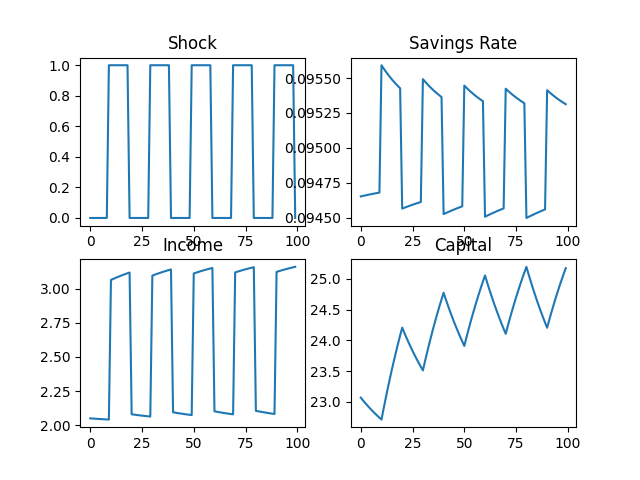
\includegraphics[scale=0.6]{\dir/capital_planner_IR_July17_1.png}
		\end{figure}
	
		\item 2 houeholds, 1 capital (4 state variables)
		
					\begin{figure}
			\centering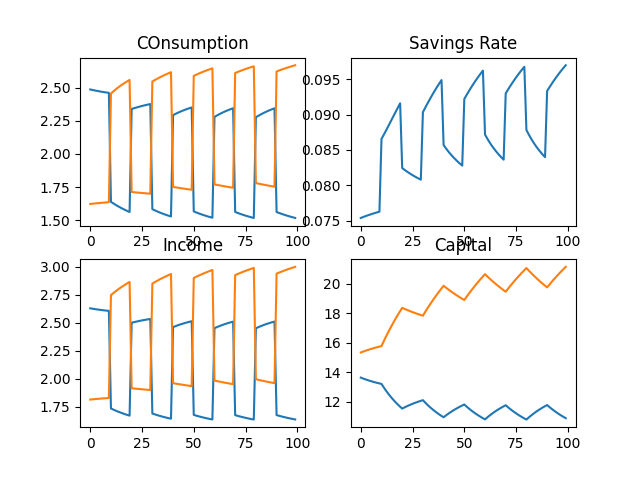
\includegraphics[scale=0.6]{\dir/capital_planner_IR_July17_2.png}
		\end{figure}
	
			\item Comparison with optimal path
	
	\begin{figure}
		\centering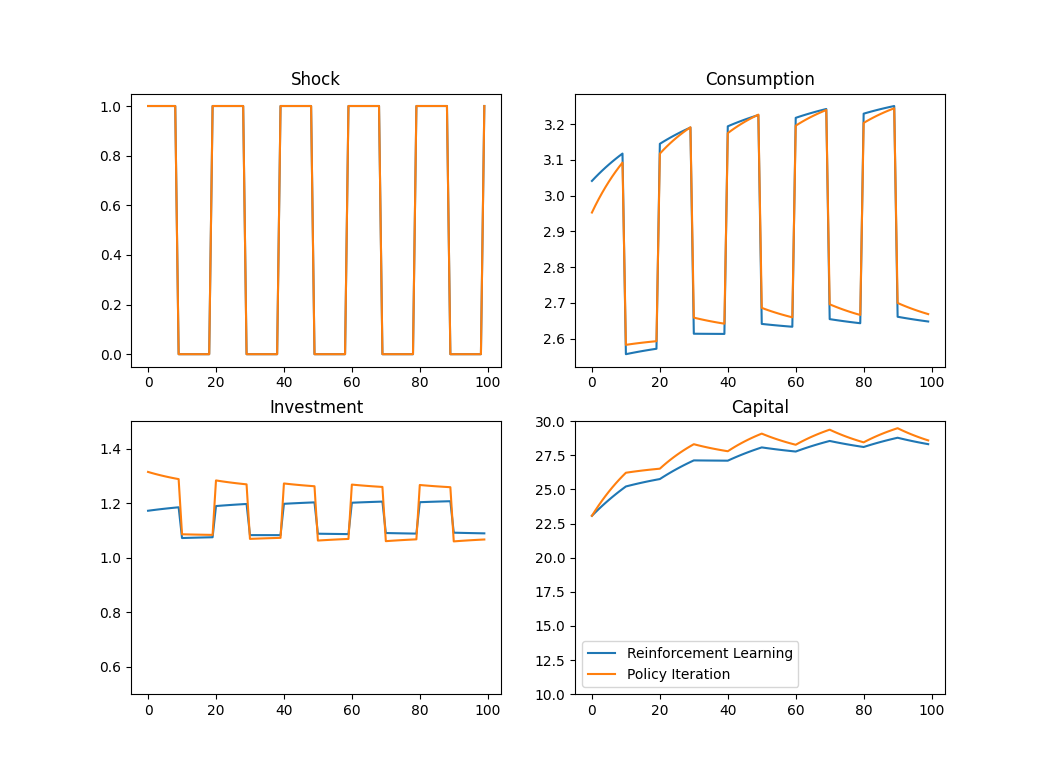
\includegraphics[scale=0.6]{\dir/econ_v_srl_1hh_July29.png}
	\end{figure}
	
		
		
	\end{itemize}


	\item Exercise 2: many capital goods, (1v1, 2v2, 10v10)
\end{itemize}

\subsection{Multi-agent learning}
\begin{itemize}
	\item Explain centralized critic algorithm.
	\item Explain parallelized computation framework.
	\item Exercise 1: 1 vs 5 vs 100 households.
	\item Exercise 2: Capital Good firms as AI agents. 1 vs 1, 2 vs 2, 10 vs 10. Does it converge to competitive equilibrium?	
	\item Exercise 3: Half the households have full info and half the households only observe own and aggregate stock.
\end{itemize}


\section{Design Lessons}
\begin{itemize}
	\item Exercise 1: Choosing spending vs choosing quantities. General normalization issues.
	\item Exercise 2: How to specify markets.
	\item Exercise 3: How to impose constrains.
	\item Exercise 3: Learning rates and algorithmic issues?
\end{itemize}

\section{Conclusion}

to be done


\bibliographystyle{plainnat}
\bibliography{MarketsAI.bib}

\end{document}
